\documentclass[main.tex]{subfiles}

\begin{document}
\lhead{Appendix}
\chapter{Figures}
\section{Dimensionality Reduction}
\label{sec:dimredu}

\begin{figure}[H]
    \centering
        % 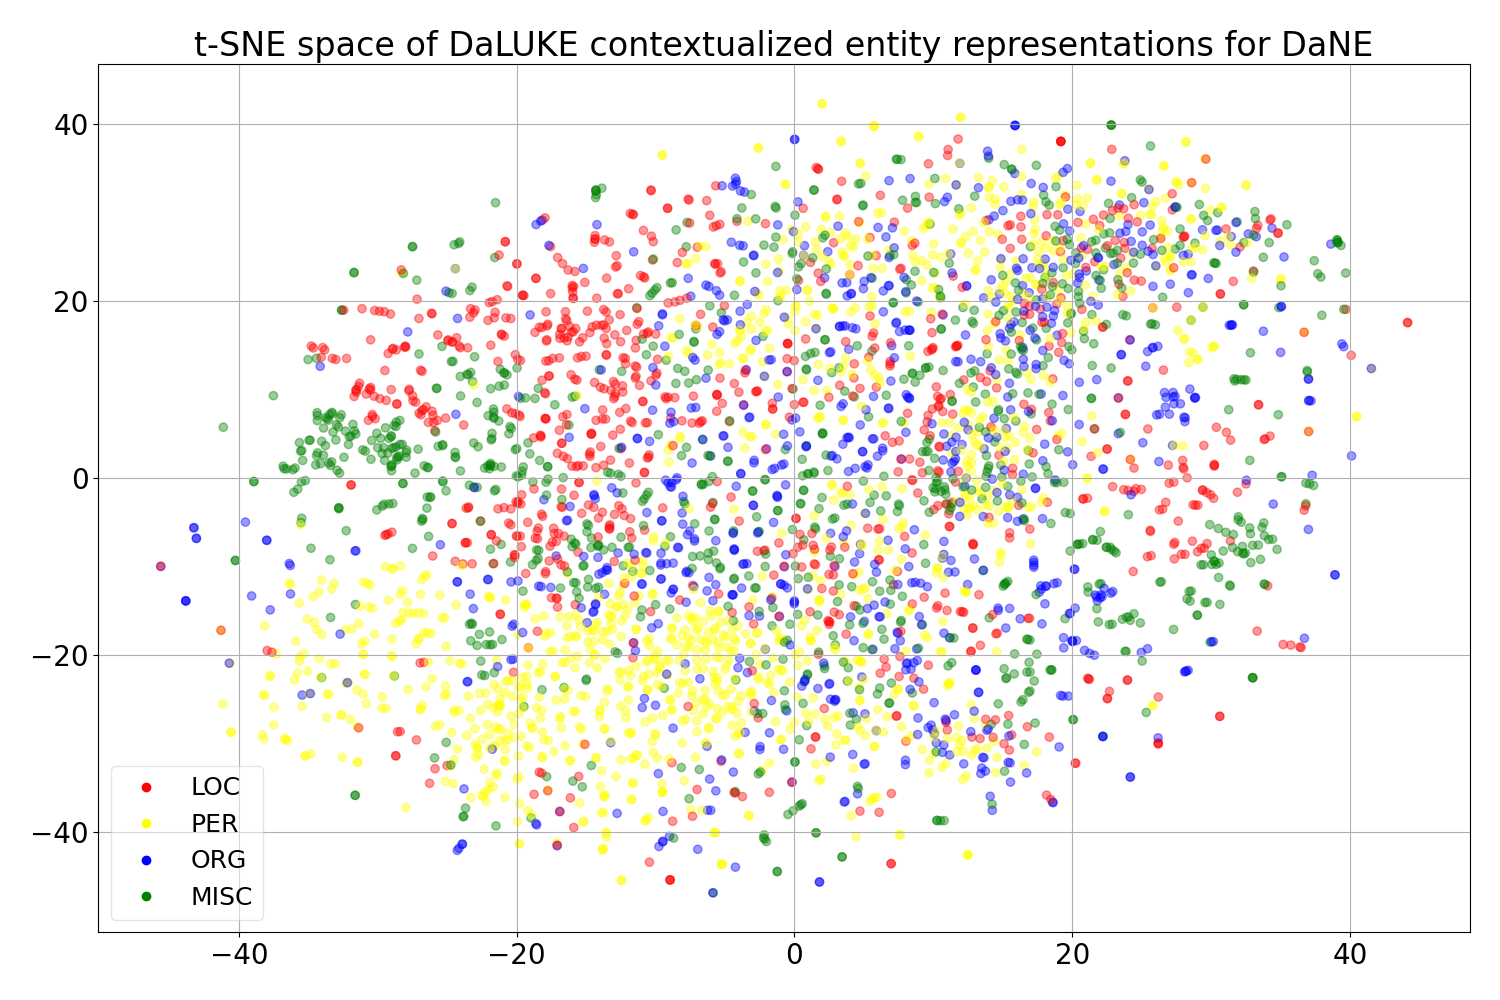
\includegraphics[width=0.7\linewidth]{full-geo/tsne}
    \caption{
        $t$-SNE performed on the full $\sim$ 1M possible entity spans in the training set of DaNE.
    }
    \label{fig:full-tsne}
\end{figure}\noindent

\begin{figure}[H]
    \centering
        % 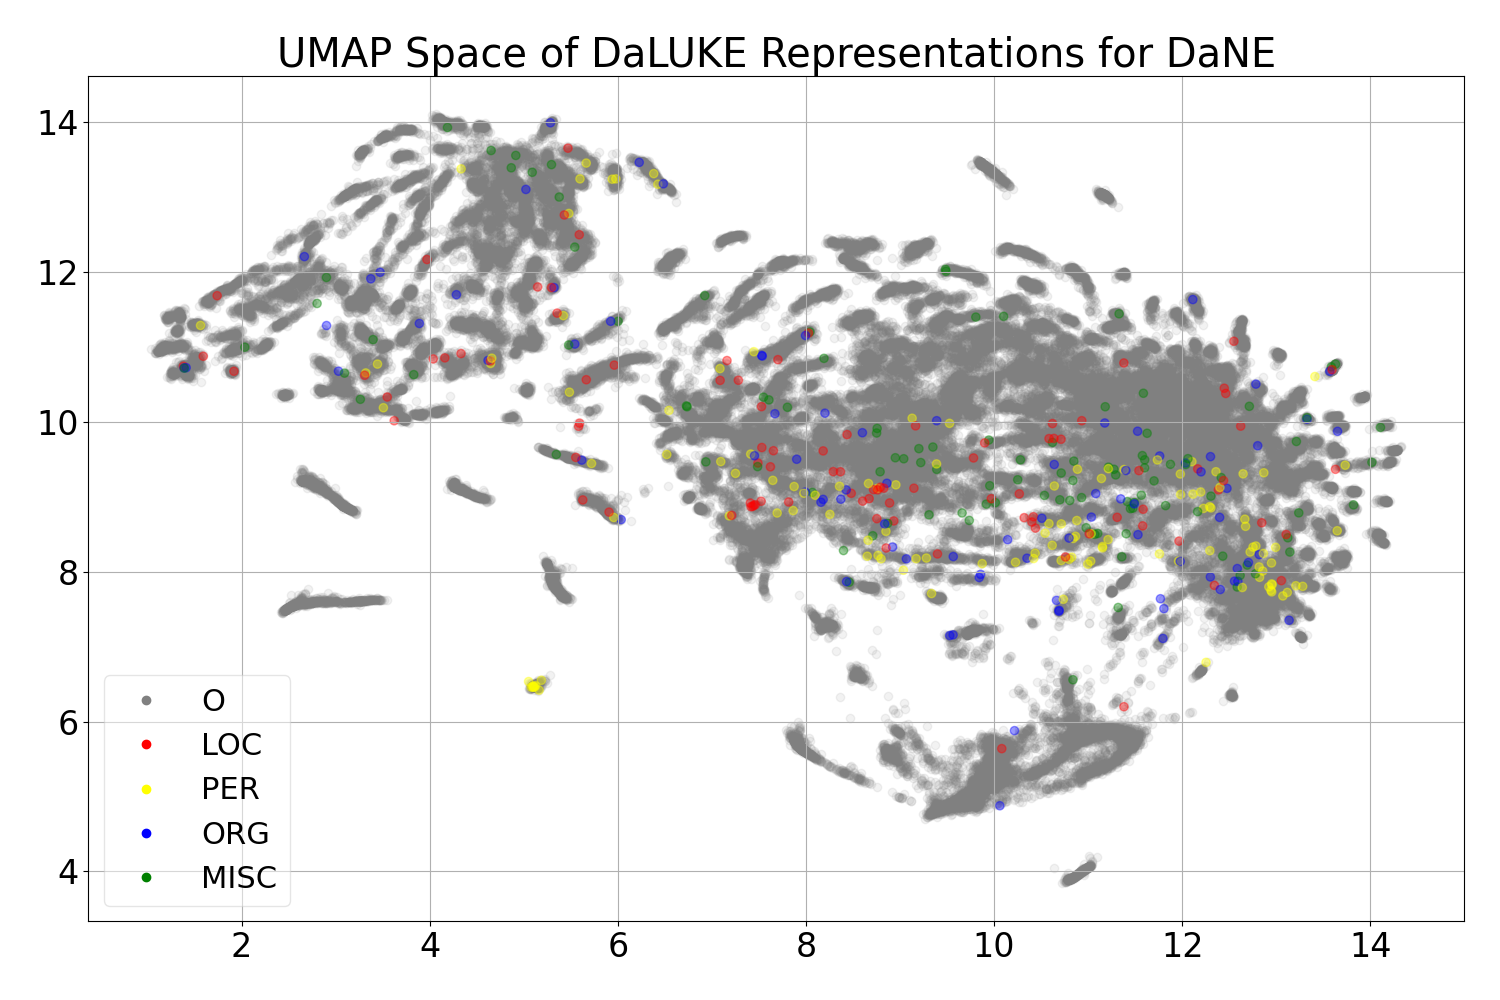
\includegraphics[width=0.7\linewidth]{full-geo/umap}
    \caption{
        UMAP performed on the full $\sim$ 1M possible entity spans in the DaNE training set.
    }
    \label{fig:full-umap}
\end{figure}\noindent

\begin{figure}[H]
    \centering
        % \includegraphics[width=\linewidth]{full-geo/variance_explained}
    \caption{
        Variance explained by principal components found by PCA on full DaNE training dataset.
    }
    \label{fig:full-varex}
\end{figure}\noindent

\begin{figure}[H]
    \centering
        % \includegraphics[width=\linewidth]{full-geo/variance_explained}
    \caption{
        Variance explained by principal components found by PCA on the full dataset.
    }
    \label{fig:full-varex}
\end{figure}\noindent

\begin{figure}[H]
    \centering
        \includegraphics[width=\linewidth]{pos-geo/variance_explained}
    \caption{
        Variance explained by principal components found by PCA on the dataset including positive labels.
    }
    \label{fig:pos-varex}
\end{figure}\noindent

\end{document}
